% Options for packages loaded elsewhere
\PassOptionsToPackage{unicode}{hyperref}
\PassOptionsToPackage{hyphens}{url}
\PassOptionsToPackage{dvipsnames,svgnames,x11names}{xcolor}
%
\documentclass[
  letterpaper,
  DIV=11,
  numbers=noendperiod]{scrartcl}

\usepackage{amsmath,amssymb}
\usepackage{iftex}
\ifPDFTeX
  \usepackage[T1]{fontenc}
  \usepackage[utf8]{inputenc}
  \usepackage{textcomp} % provide euro and other symbols
\else % if luatex or xetex
  \usepackage{unicode-math}
  \defaultfontfeatures{Scale=MatchLowercase}
  \defaultfontfeatures[\rmfamily]{Ligatures=TeX,Scale=1}
\fi
\usepackage{lmodern}
\ifPDFTeX\else  
    % xetex/luatex font selection
\fi
% Use upquote if available, for straight quotes in verbatim environments
\IfFileExists{upquote.sty}{\usepackage{upquote}}{}
\IfFileExists{microtype.sty}{% use microtype if available
  \usepackage[]{microtype}
  \UseMicrotypeSet[protrusion]{basicmath} % disable protrusion for tt fonts
}{}
\makeatletter
\@ifundefined{KOMAClassName}{% if non-KOMA class
  \IfFileExists{parskip.sty}{%
    \usepackage{parskip}
  }{% else
    \setlength{\parindent}{0pt}
    \setlength{\parskip}{6pt plus 2pt minus 1pt}}
}{% if KOMA class
  \KOMAoptions{parskip=half}}
\makeatother
\usepackage{xcolor}
\setlength{\emergencystretch}{3em} % prevent overfull lines
\setcounter{secnumdepth}{-\maxdimen} % remove section numbering
% Make \paragraph and \subparagraph free-standing
\ifx\paragraph\undefined\else
  \let\oldparagraph\paragraph
  \renewcommand{\paragraph}[1]{\oldparagraph{#1}\mbox{}}
\fi
\ifx\subparagraph\undefined\else
  \let\oldsubparagraph\subparagraph
  \renewcommand{\subparagraph}[1]{\oldsubparagraph{#1}\mbox{}}
\fi


\providecommand{\tightlist}{%
  \setlength{\itemsep}{0pt}\setlength{\parskip}{0pt}}\usepackage{longtable,booktabs,array}
\usepackage{calc} % for calculating minipage widths
% Correct order of tables after \paragraph or \subparagraph
\usepackage{etoolbox}
\makeatletter
\patchcmd\longtable{\par}{\if@noskipsec\mbox{}\fi\par}{}{}
\makeatother
% Allow footnotes in longtable head/foot
\IfFileExists{footnotehyper.sty}{\usepackage{footnotehyper}}{\usepackage{footnote}}
\makesavenoteenv{longtable}
\usepackage{graphicx}
\makeatletter
\def\maxwidth{\ifdim\Gin@nat@width>\linewidth\linewidth\else\Gin@nat@width\fi}
\def\maxheight{\ifdim\Gin@nat@height>\textheight\textheight\else\Gin@nat@height\fi}
\makeatother
% Scale images if necessary, so that they will not overflow the page
% margins by default, and it is still possible to overwrite the defaults
% using explicit options in \includegraphics[width, height, ...]{}
\setkeys{Gin}{width=\maxwidth,height=\maxheight,keepaspectratio}
% Set default figure placement to htbp
\makeatletter
\def\fps@figure{htbp}
\makeatother
\newlength{\cslhangindent}
\setlength{\cslhangindent}{1.5em}
\newlength{\csllabelwidth}
\setlength{\csllabelwidth}{3em}
\newlength{\cslentryspacingunit} % times entry-spacing
\setlength{\cslentryspacingunit}{\parskip}
\newenvironment{CSLReferences}[2] % #1 hanging-ident, #2 entry spacing
 {% don't indent paragraphs
  \setlength{\parindent}{0pt}
  % turn on hanging indent if param 1 is 1
  \ifodd #1
  \let\oldpar\par
  \def\par{\hangindent=\cslhangindent\oldpar}
  \fi
  % set entry spacing
  \setlength{\parskip}{#2\cslentryspacingunit}
 }%
 {}
\usepackage{calc}
\newcommand{\CSLBlock}[1]{#1\hfill\break}
\newcommand{\CSLLeftMargin}[1]{\parbox[t]{\csllabelwidth}{#1}}
\newcommand{\CSLRightInline}[1]{\parbox[t]{\linewidth - \csllabelwidth}{#1}\break}
\newcommand{\CSLIndent}[1]{\hspace{\cslhangindent}#1}

\usepackage{booktabs}
\usepackage{longtable}
\usepackage{array}
\usepackage{multirow}
\usepackage{wrapfig}
\usepackage{float}
\usepackage{colortbl}
\usepackage{pdflscape}
\usepackage{tabu}
\usepackage{threeparttable}
\usepackage{threeparttablex}
\usepackage[normalem]{ulem}
\usepackage{makecell}
\usepackage{xcolor}
\KOMAoption{captions}{tableheading}
\makeatletter
\makeatother
\makeatletter
\makeatother
\makeatletter
\@ifpackageloaded{caption}{}{\usepackage{caption}}
\AtBeginDocument{%
\ifdefined\contentsname
  \renewcommand*\contentsname{Table of contents}
\else
  \newcommand\contentsname{Table of contents}
\fi
\ifdefined\listfigurename
  \renewcommand*\listfigurename{List of Figures}
\else
  \newcommand\listfigurename{List of Figures}
\fi
\ifdefined\listtablename
  \renewcommand*\listtablename{List of Tables}
\else
  \newcommand\listtablename{List of Tables}
\fi
\ifdefined\figurename
  \renewcommand*\figurename{Figure}
\else
  \newcommand\figurename{Figure}
\fi
\ifdefined\tablename
  \renewcommand*\tablename{Table}
\else
  \newcommand\tablename{Table}
\fi
}
\@ifpackageloaded{float}{}{\usepackage{float}}
\floatstyle{ruled}
\@ifundefined{c@chapter}{\newfloat{codelisting}{h}{lop}}{\newfloat{codelisting}{h}{lop}[chapter]}
\floatname{codelisting}{Listing}
\newcommand*\listoflistings{\listof{codelisting}{List of Listings}}
\makeatother
\makeatletter
\@ifpackageloaded{caption}{}{\usepackage{caption}}
\@ifpackageloaded{subcaption}{}{\usepackage{subcaption}}
\makeatother
\makeatletter
\@ifpackageloaded{tcolorbox}{}{\usepackage[skins,breakable]{tcolorbox}}
\makeatother
\makeatletter
\@ifundefined{shadecolor}{\definecolor{shadecolor}{rgb}{.97, .97, .97}}
\makeatother
\makeatletter
\makeatother
\makeatletter
\makeatother
\ifLuaTeX
  \usepackage{selnolig}  % disable illegal ligatures
\fi
\IfFileExists{bookmark.sty}{\usepackage{bookmark}}{\usepackage{hyperref}}
\IfFileExists{xurl.sty}{\usepackage{xurl}}{} % add URL line breaks if available
\urlstyle{same} % disable monospaced font for URLs
\hypersetup{
  pdftitle={assignment\_1},
  pdfauthor={Marius Martinussen, Espen Knutsen},
  colorlinks=true,
  linkcolor={blue},
  filecolor={Maroon},
  citecolor={Blue},
  urlcolor={Blue},
  pdfcreator={LaTeX via pandoc}}

\title{assignment\_1}
\author{Marius Martinussen, Espen Knutsen}
\date{}

\begin{document}
\maketitle
\ifdefined\Shaded\renewenvironment{Shaded}{\begin{tcolorbox}[breakable, interior hidden, borderline west={3pt}{0pt}{shadecolor}, sharp corners, boxrule=0pt, enhanced, frame hidden]}{\end{tcolorbox}}\fi

\hypertarget{part-a-sub-national-gdp-and-gdp-per-capita}{%
\subsection{Part A: Sub-national GDP and GDP per
capita}\label{part-a-sub-national-gdp-and-gdp-per-capita}}

\hypertarget{data-acquisition}{%
\subsubsection{1. Data acquisition}\label{data-acquisition}}

By using Eurostat, we have downloaded data containing GDP and population
for each country in the EU from year 1990 to 2023. However, we are only
interested in the following countries from 2000 to 2020:

\hypertarget{countries-of-interest}{%
\subsubsection{Countries of interest}\label{countries-of-interest}}

\begin{itemize}
\tightlist
\item
  Italy
\item
  Sweden
\item
  Belgium
\item
  Austria
\item
  Croatia
\item
  Serbia
\item
  Bosnia and Herzegovina
\item
  Bulgaria
\end{itemize}

Below is a short extract of the raw datasets from Eurostat.

\begin{verbatim}
# A tibble: 253,544 x 8
  DATAFLOW        `LAST UPDATE` freq  unit  geo   TIME_PERIOD OBS_VALUE OBS_FLAG
  <chr>           <chr>         <chr> <chr> <chr>       <dbl>     <dbl> <chr>   
1 ESTAT:NAMA_10R~ 21/02/23 23:~ A     EUR_~ AL           2008      3000 ""      
2 ESTAT:NAMA_10R~ 21/02/23 23:~ A     EUR_~ AL           2009      3000 ""      
3 ESTAT:NAMA_10R~ 21/02/23 23:~ A     EUR_~ AL           2010      3100 ""      
4 ESTAT:NAMA_10R~ 21/02/23 23:~ A     EUR_~ AL           2011      3200 ""      
5 ESTAT:NAMA_10R~ 21/02/23 23:~ A     EUR_~ AL           2012      3300 ""      
# i 253,539 more rows
\end{verbatim}

\begin{verbatim}
# A tibble: 649,023 x 10
  DATAFLOW     `LAST UPDATE` freq  unit  sex   age   geo   TIME_PERIOD OBS_VALUE
  <chr>        <chr>         <chr> <chr> <chr> <chr> <chr>       <dbl>     <dbl>
1 ESTAT:DEMO_~ 28/09/23 23:~ A     NR    F     TOTAL AL           2000   1526762
2 ESTAT:DEMO_~ 28/09/23 23:~ A     NR    F     TOTAL AL           2001   1535822
3 ESTAT:DEMO_~ 28/09/23 23:~ A     NR    F     TOTAL AL           2002   1532563
4 ESTAT:DEMO_~ 28/09/23 23:~ A     NR    F     TOTAL AL           2003   1526180
5 ESTAT:DEMO_~ 28/09/23 23:~ A     NR    F     TOTAL AL           2004   1520481
# i 649,018 more rows
# i 1 more variable: OBS_FLAG <chr>
\end{verbatim}

-\/-\/-\/-\/-\/-\/-\/-\/-\/-\/-\/-\/-\/-\/-\/-\/-\/-\/-\/-\/-\/-\/-\/-\/-\/-\/-\/-\/-\/-\/-\/-\/-\/-\/-\/-\/-\/-\/-\/-\/-\/-\/-\/-\/-\/-\/-\/-\/-\/-\/-\/-\/-\/-\/-\/-\/-\/-\/-\/-\/-\/-\/-\/-\/-\/-\/-\/-\/-

\hypertarget{description}{%
\subsection{Description}\label{description}}

In order to substract the countries in focus, we have used the metadata
provided by Eurostat to filter out the data and variables of interest,
using their respective country codes. The variables we are interested in
are the following:

\begin{itemize}
\tightlist
\item
  geo = Tells us which country and sub-region we are looking at
\item
  time\_period = Observed years
\item
  obs\_value = The value of the observation
\item
  Unit = Currency
\end{itemize}

By filtering out irrelevant data and variables and rearranging the
dataset to provide a clearer view, results with the following datasets:

\begin{verbatim}
# A tibble: 5,398 x 3
   year geo     GDP
  <dbl> <chr> <dbl>
1  2000 AT111  597.
2  2001 AT111  627.
3  2002 AT111  627.
4  2003 AT111  675.
5  2004 AT111  676.
# i 5,393 more rows
\end{verbatim}

\begin{verbatim}
# A tibble: 5,441 x 3
   year geo   Population
  <dbl> <chr>      <dbl>
1  2001 AT111      37732
2  2002 AT111      37778
3  2003 AT111      37703
4  2004 AT111      37640
5  2005 AT111      37522
# i 5,436 more rows
\end{verbatim}

\hypertarget{gdp-per-capita-calculation}{%
\subsubsection{2. GDP per capita
calculation}\label{gdp-per-capita-calculation}}

In order to visualize the GDP per capita, we have merged the two
datasets together and added a new variable that executes this formula in
order to generate the GDP per capita for every country.

\(y_i = \frac{\text{GDP}_i}{\text{population}_i}\)

It is worth noting that the GDP data from Eurostat is represented in
million euros,, meaning that 1 in this case, equals 1 million euros. 0.1
represent 100 000 euros, and so on. This will be consistent through all
our visualized data.

GDP or Gross Domestic Product is a measure of value creation in a
country. This is described by Eurostat to be ``a measure of economic
activity, defined as the value of all goods and services produced minus
the value of any goods or services used in their creation''Eurostat
(2023). How Eurostat calculates the annual growth rate in GDP
``comparisons of the dynamics of economic development both over time and
between economies of different sizes''Eurostat (2023). To measure the
growth rate of GDP over time ``in volume, GDP in current prices is
valued at the prices of the previous year, and the volume changes thus
calculated are imposed on the level of a reference year; this is called
a chain-linked series. Consequently, price movements will not inflate
growth''Eurostat (2023).

\hypertarget{descriptive-analysis}{%
\subsubsection{3. Descriptive analysis}\label{descriptive-analysis}}

\hypertarget{austria}{%
\subsubsection{Austria}\label{austria}}

\includegraphics{assignment_1_files/figure-pdf/unnamed-chunk-11-1.pdf}

\begin{table}

\caption{Summary Statistics}
\centering
\begin{tabular}[t]{lllllllll}
\toprule
Variable & N & Mean & Std. Dev. & Min & Pctl. 25 & Pctl. 50 & Pctl. 75 & Max\\
\midrule
GDP_pc_n3 & 701 & 32066 & 9542 & 14236 & 24563 & 30679 & 38835 & 57760\\
\bottomrule
\end{tabular}
\end{table}

Outliers: None

The sub-regions follow the same trends in GDP per per capita, with
certain exceptions linked to a marked decrease in AT331 (Außerfern) in
connection with 2008 (the financial crisis). This may be due to the fact
that this is an administrative district, and is often more exposed to a
financial crisis.

All sub-regions have a decline in GDP per per capita from 2019 -- 2020
in connection with covid 19, where some sub-regions have a more marked
decline than others. This probably has a natural explanation in how the
guidelines were followed through covid and how much the individual
sub-region's gdp per capita depends on tourism.

In summary of the data set, Austria has a minimum value and a maximum
value of 14,236 and 57,760 gdp per year, respectively. capita, with a
standard deviation of 9542. This standard deviation measures how much
spread or variance there is in the values in the data set. Furthermore,
the data set has an average of 32,066 GDP per capita, with a median of
30,679 GDP per capita. When the median is lower than the mean, this
means that the data set has more values closer to the minimum value in
the data set.

\hypertarget{belgium}{%
\subsubsection{Belgium}\label{belgium}}

\includegraphics{assignment_1_files/figure-pdf/unnamed-chunk-13-1.pdf}

\begin{table}

\caption{Summary Statistics}
\centering
\begin{tabular}[t]{lllllllll}
\toprule
Variable & N & Mean & Std. Dev. & Min & Pctl. 25 & Pctl. 50 & Pctl. 75 & Max\\
\midrule
GDP_pc_n3 & 662 & 29182 & 10143 & 12756 & 22307 & 27132 & 34650 & 71959\\
\bottomrule
\end{tabular}
\end{table}

The data set shows us that we have an outliers in the form of BE100
(Brussels) which has a significantly higher GDP per capita. This has a
natural connection with the fact that Brussels is the capital of
Belgium, and has a higher traffic for trade than the other sub-regions.

Summarized by the data set, Belgium has a minimum value and a maximum
value of 12756 and 71959 gdp per year respectively. capita, with a
standard deviation of 10143. This standard deviation measures how much
spread or variance there is in the values in the data set. Furthermore,
the data set has an average of 29,182 GDP per capita, with a median of
27,132 GDP per capita. When the median is lower than the mean, this
means that the data set has more values closer to the minimum value in
the data set.

\hypertarget{bulgaria}{%
\subsubsection{Bulgaria}\label{bulgaria}}

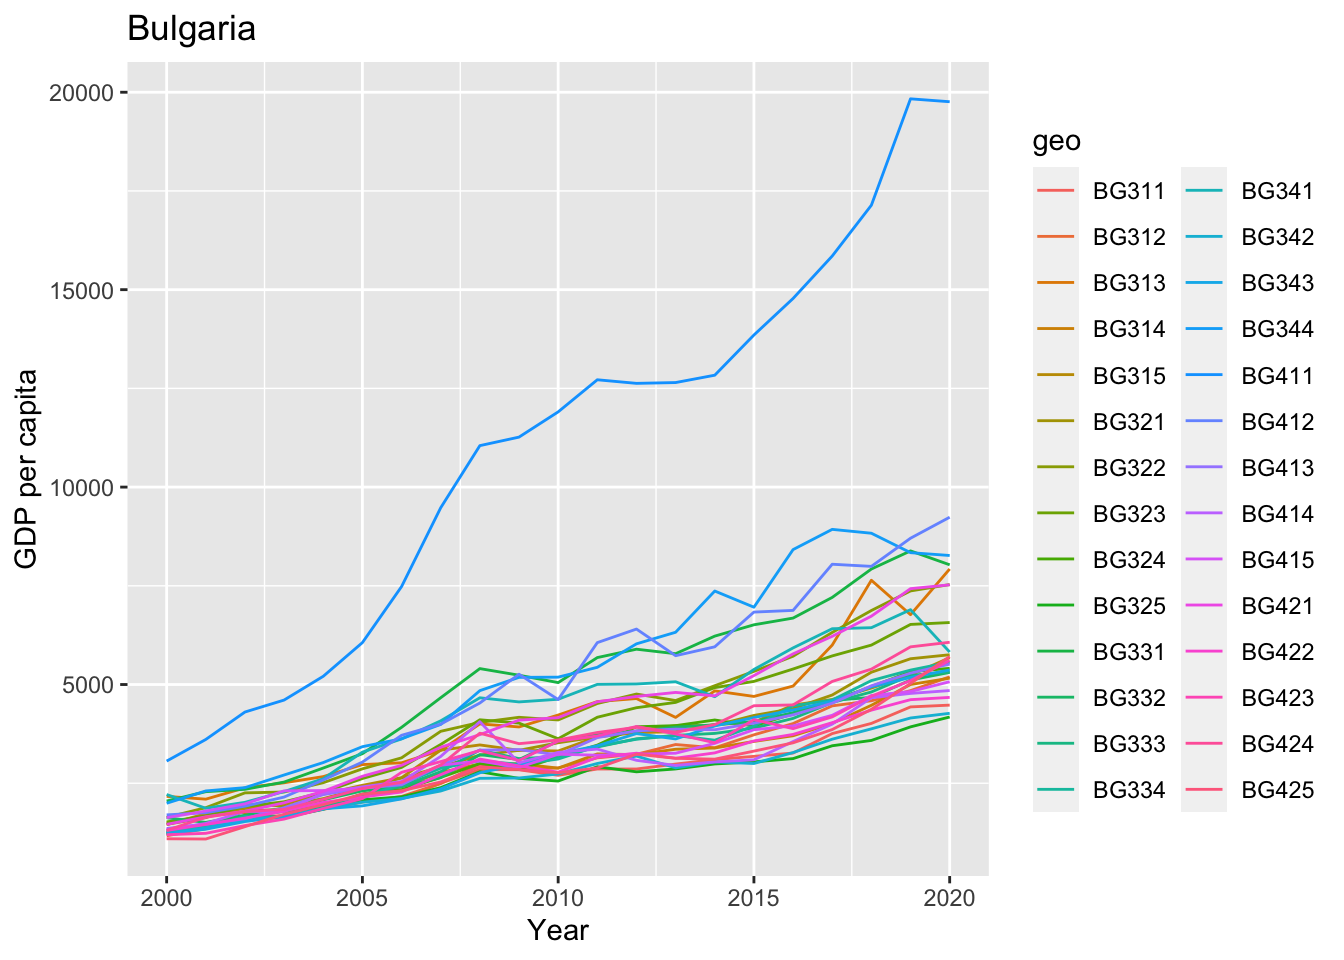
\includegraphics{assignment_1_files/figure-pdf/unnamed-chunk-15-1.pdf}

\begin{table}

\caption{Summary Statistics}
\centering
\begin{tabular}[t]{lllllllll}
\toprule
Variable & N & Mean & Std. Dev. & Min & Pctl. 25 & Pctl. 50 & Pctl. 75 & Max\\
\midrule
GDP_pc_n3 & 588 & 3826 & 2283 & 1087 & 2364 & 3378 & 4610 & 19833\\
\bottomrule
\end{tabular}
\end{table}

The explanation behind the significantly higher GDP per capita. capita
in Sofia is that it is the capital of Bulgaria and is the
administrative, cultural and economic center of the country.

Summarized by the data set, Bulgaria has a minimum value and a maximum
value of 1087 and 19833 GDP per year respectively. capita, with a
standard deviation of 2283. This standard deviation measures how much
spread or variance there is in the values in the data set. Furthermore,
the dataset has an average of 3826 GDP per capita, with a median of 3378
GDP per capita. When the median is lower than the mean, this means that
the data set has more values closer to the minimum value in the data
set.

Italy

The reason why we divide Italy into north and south is because it makes
our ggplot more clear.

\hypertarget{north-italy}{%
\subsubsection{North Italy}\label{north-italy}}

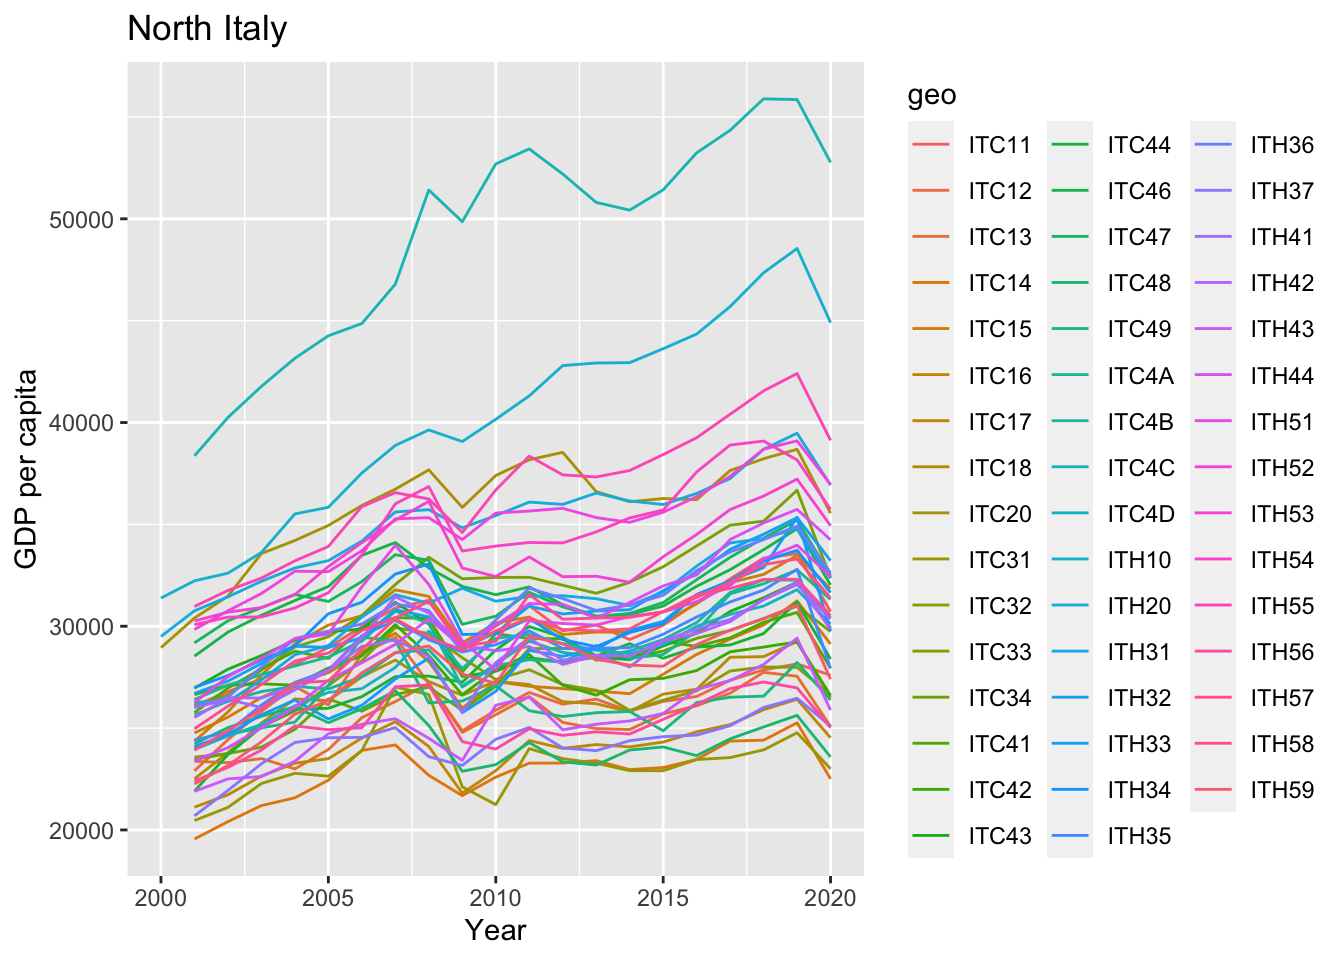
\includegraphics{assignment_1_files/figure-pdf/unnamed-chunk-17-1.pdf}

\begin{table}

\caption{Summary Statistics}
\centering
\begin{tabular}[t]{lllllllll}
\toprule
Variable & N & Mean & Std. Dev. & Min & Pctl. 25 & Pctl. 50 & Pctl. 75 & Max\\
\midrule
GDP_pc_n3 & 943 & 29733 & 5107 & 19555 & 26427 & 29097 & 31765 & 55890\\
\bottomrule
\end{tabular}
\end{table}

Outliers: ITC4C (milano) og til dels ITH10 (boltzano)

In summary of the data set, Northern Italy has a minimum value and a
maximum value of 19,555 and 55,890 gdp respectively. capita, with a
standard deviation of 5107. This standard deviation measures how much
spread or variance there is in the values in the data set. Furthermore,
the dataset has an average of 29,733 GDP per capita, with a median of
29,097 GDP per capita. When the median is higher than the mean, this
means that the data set has more values closer to the maximum value in
the data set.

\hypertarget{south-italy}{%
\subsubsection{South Italy}\label{south-italy}}

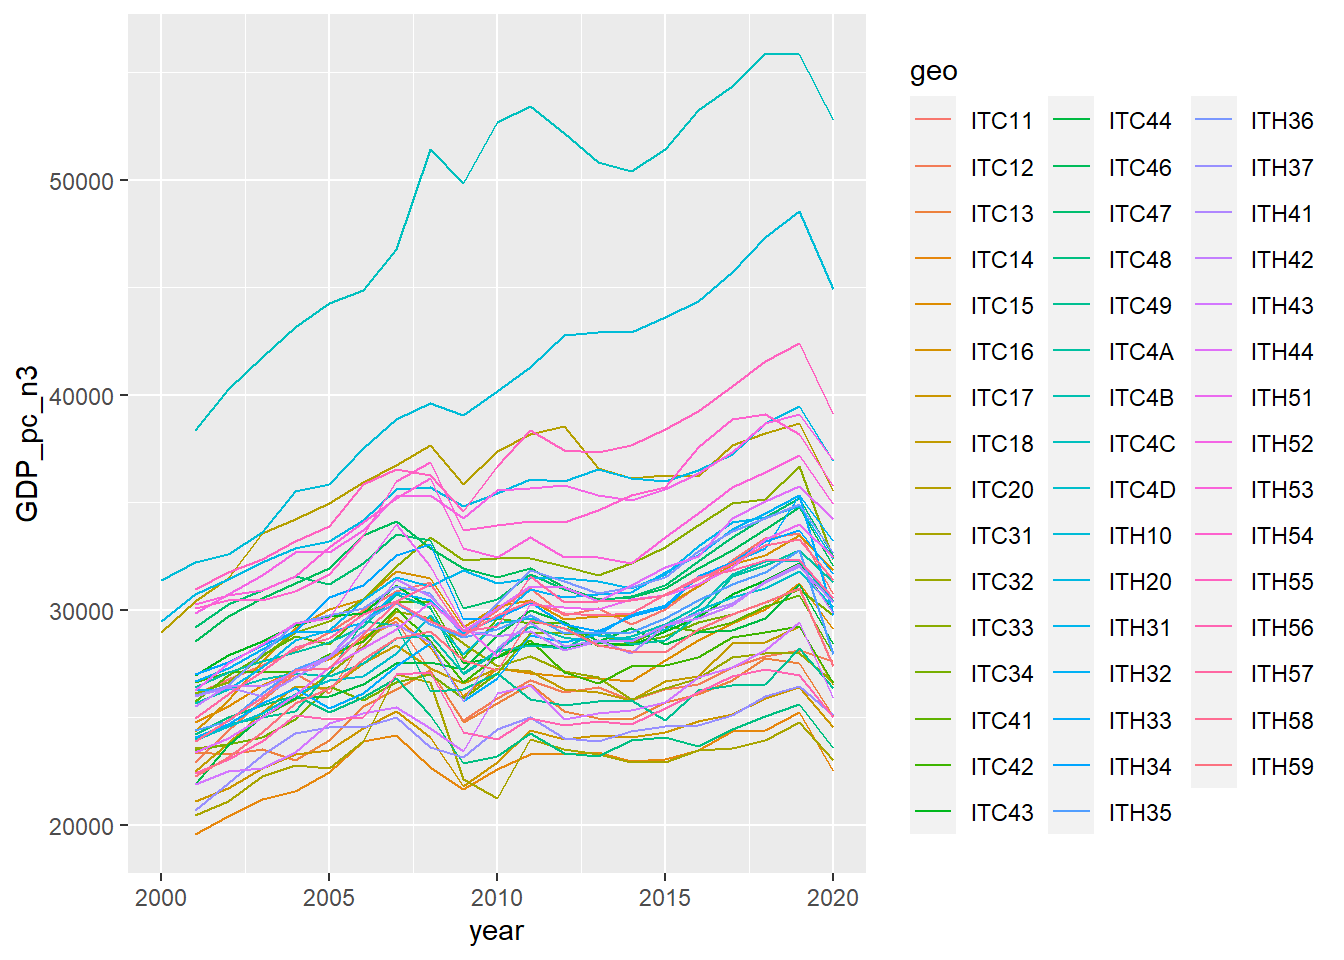
\includegraphics{assignment_1_files/figure-pdf/unnamed-chunk-19-1.pdf}

\begin{table}

\caption{Summary Statistics}
\centering
\begin{tabular}[t]{lllllllll}
\toprule
Variable & N & Mean & Std. Dev. & Min & Pctl. 25 & Pctl. 50 & Pctl. 75 & Max\\
\midrule
GDP_pc_n3 & 1100 & 20995 & 5302 & 11713 & 16889 & 19788 & 24334 & 42801\\
\bottomrule
\end{tabular}
\end{table}

Outliers: ITI14(Chieti), ITI43(Taranto).

Summarized by the data set, Southern Italy has a minimum value and a
maximum value of 11713 and 42801 gdp per year respectively. capita, with
a standard deviation of 5302. This standard deviation measures how much
spread or variance there is in the values in the data set. Furthermore,
the data set has an average of 20995 GDP per capita, with a median of
19788 GDP per capita. When the median is lower than the mean, this means
that the data set has more values closer to the minimum value in the
data set.

\hypertarget{sweden}{%
\subsubsection{Sweden}\label{sweden}}

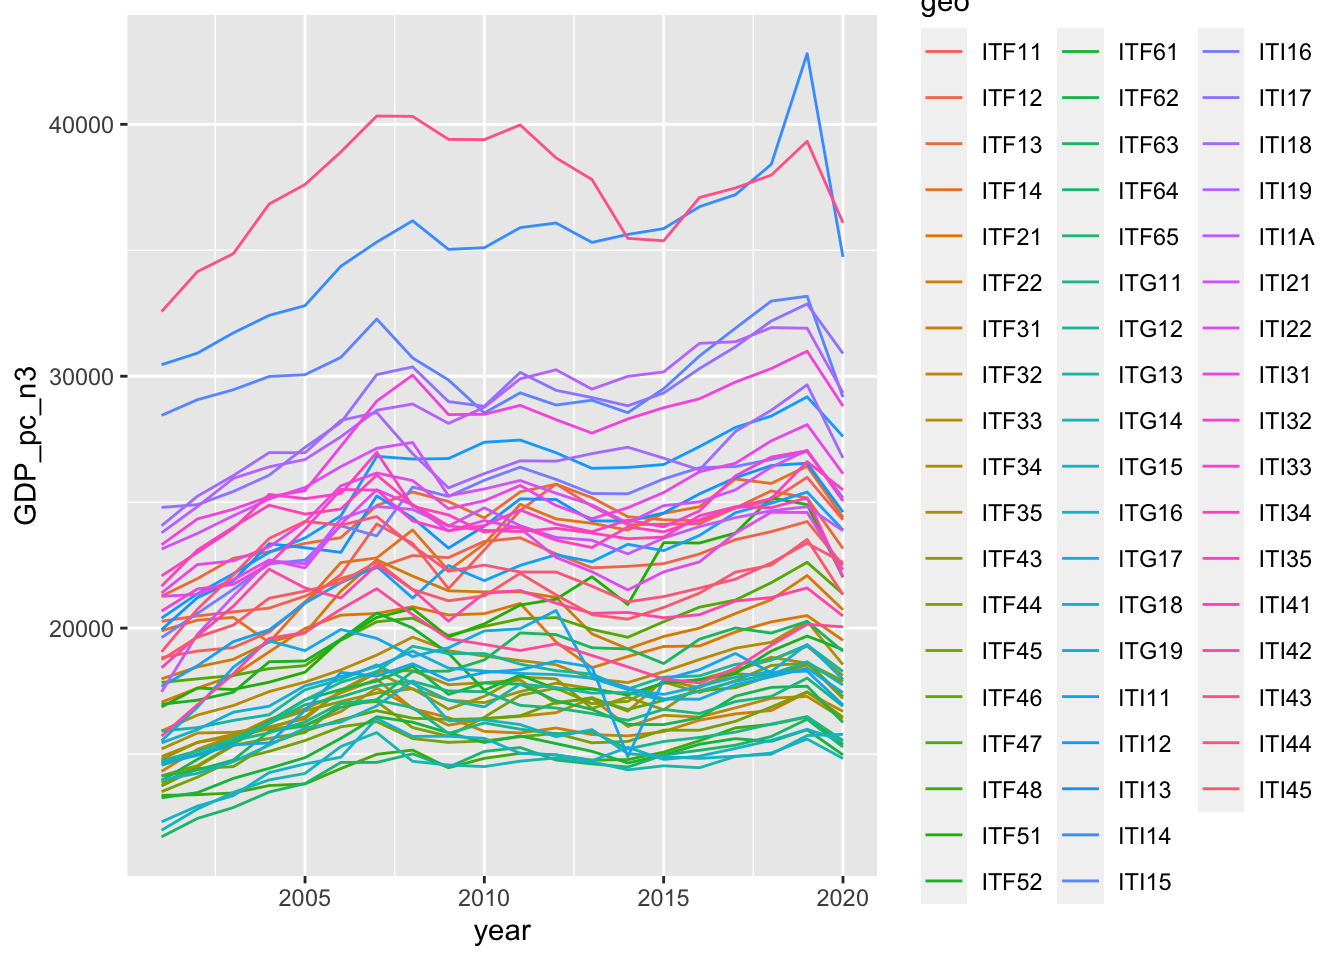
\includegraphics{assignment_1_files/figure-pdf/unnamed-chunk-21-1.pdf}

\begin{table}

\caption{Summary Statistics}
\centering
\begin{tabular}[t]{lllllllll}
\toprule
Variable & N & Mean & Std. Dev. & Min & Pctl. 25 & Pctl. 50 & Pctl. 75 & Max\\
\midrule
GDP_pc_n3 & 441 & 35757 & 7515 & 23331 & 30110 & 35308 & 39550 & 66250\\
\bottomrule
\end{tabular}
\end{table}

Sweden: We have an extreme value in the form of a significantly higher
GDP per capita in sub region SE110 which is Stockholm. This can be
explained by the fact that it is the capital and it is natural that
value creation is centralized around Stockholm.

The data shows that there is a fall in GDP per capita throughout Sweden
in 2008. The natural explanation for this would be the financial crisis
in 2008.

The data also shows a reduction in 2019 - 2020 in many sub-regions that
can be linked to covid 19. The reason why not all sub-regions had this
drop may be that large parts of Sweden did not comply with the
restrictions linked to the infection of the virus.

Summarized by the data set, Sweden has a minimum value and a maximum
value of 23331 and 66250 GDP per year respectively. capita, with a
standard deviation of 7515. This standard deviation measures how much
spread or variance there is in the values in the data set. Furthermore,
the data set has an average of 35,757 GDP per capita, with a median of
39,550 GDP per capita. When the median is higher than the mean, this
means that the data set has more values closer to the maximum value in
the data set.

\hypertarget{croatia---became-a-member-in-2012}{%
\subsubsection{Croatia - became a member in
2012}\label{croatia---became-a-member-in-2012}}

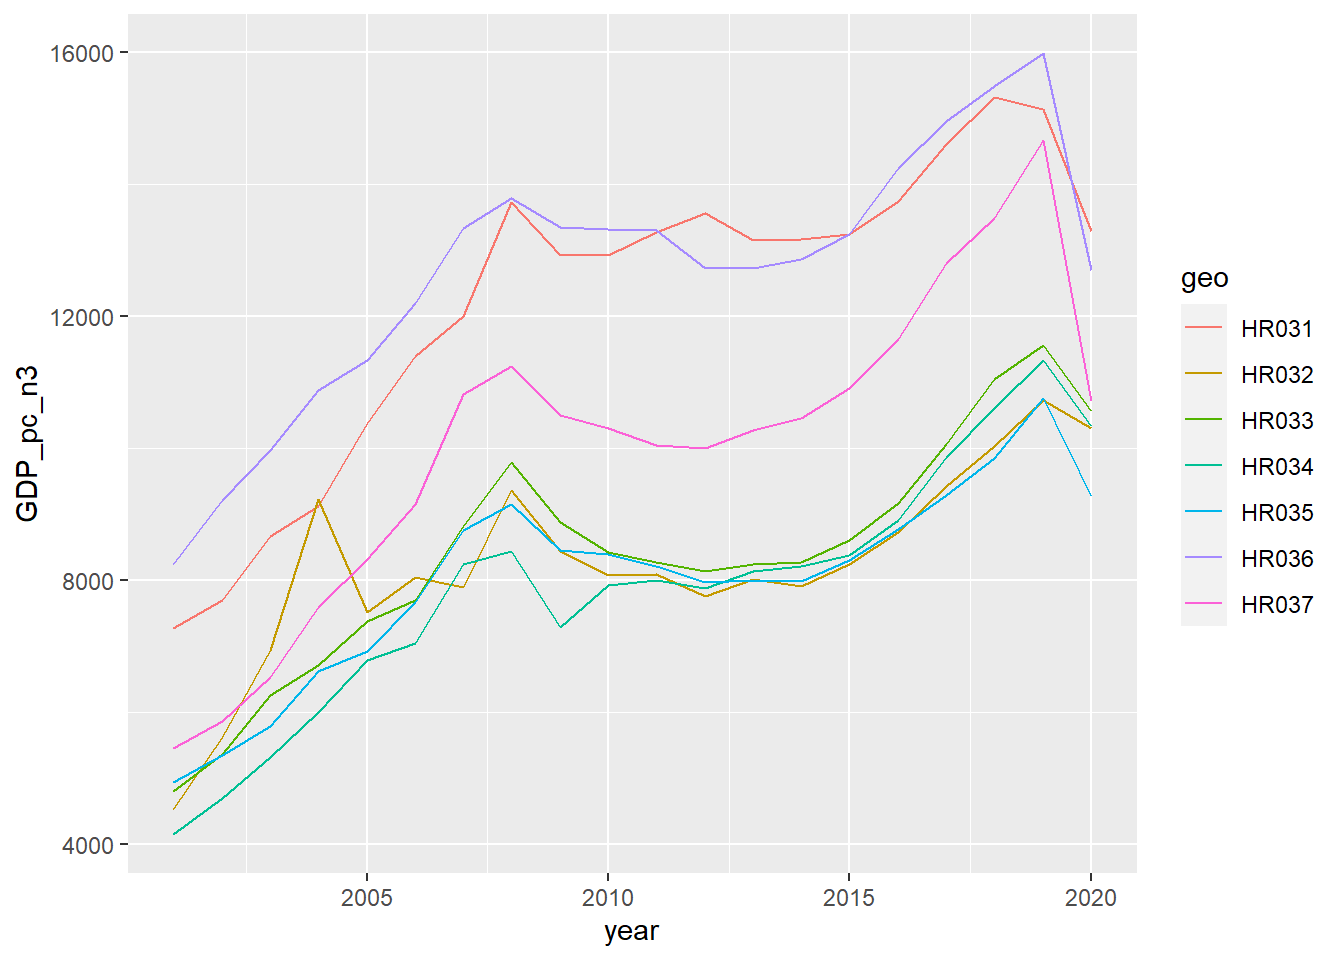
\includegraphics{assignment_1_files/figure-pdf/unnamed-chunk-23-1.pdf}

\begin{table}

\caption{Summary Statistics}
\centering
\begin{tabular}[t]{lllllllll}
\toprule
Variable & N & Mean & Std. Dev. & Min & Pctl. 25 & Pctl. 50 & Pctl. 75 & Max\\
\midrule
GDP_pc_n3 & 140 & 9644 & 2692 & 4144 & 7981 & 9155 & 11355 & 15985\\
\bottomrule
\end{tabular}
\end{table}

From the data set we see that Croatia are missing populationdata in the
subregions HR050, HR061- HR065 and HR021 - HR028. We therefore only have
data from the subregions HR031 - HR037 to take a closer look at GDP per
capita. From the data set, we see that all the subregions have a similar
trend pattern, where the fall in GDP in 2019 - 2020 can be explained by
Covid - 19.

There are three sub regions in the form of HR031, HR036 and HR037 which
are Primorsko Goranska, Istrian and Dubrovnik-Neretva stand out with a
higher GDP per Capita. All these sub-regions are located along the
coast, and this would likley attract tourism.

In summary of the data set, Croatia has a minimum value and a maximum
value of 4144 and 15985 GDP per year respectively. capita, with a
standard deviation of 2692. This standard deviation measures how much
spread or variance there is in the values in the data set. Furthermore,
the data set has an average of 9644 GDP per capita, with a median of
9155 GDP per capita. When the median is lower than the mean, this means
that the data set has more values closer to the minimum value in the
data set.

\hypertarget{serbia-eu-candidate-country}{%
\subsubsection{Serbia (EU candidate
country)}\label{serbia-eu-candidate-country}}

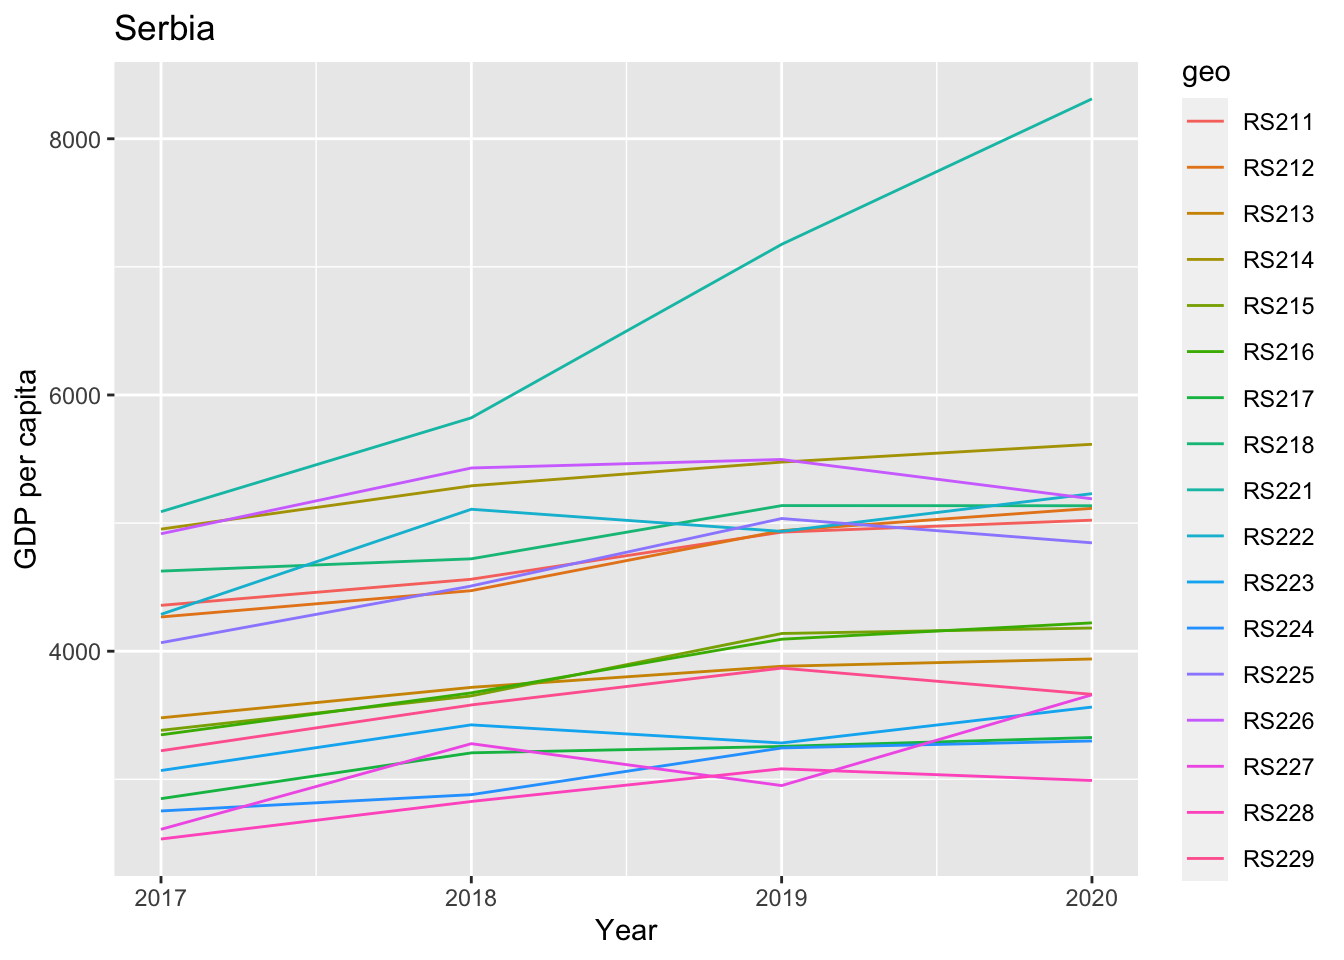
\includegraphics{assignment_1_files/figure-pdf/unnamed-chunk-25-1.pdf}

\begin{table}

\caption{Summary Statistics}
\centering
\begin{tabular}[t]{lllllllll}
\toprule
Variable & N & Mean & Std. Dev. & Min & Pctl. 25 & Pctl. 50 & Pctl. 75 & Max\\
\midrule
GDP_pc_n3 & 68 & 4209 & 1081 & 2534 & 3320 & 4116 & 4970 & 8312\\
\bottomrule
\end{tabular}
\end{table}

The reason why the dataset lacks GDP per capita in Serbia from 2000 -
2017 is explained by the fact that Serbia is an EU candidate and not
part of the EU. It is therefore partly unclear where we get data from
2017 - 2020, but can be explained by the fact that Serbia applied to
join the EU in December 2009, and received the status of ``EU
candidate'' in March 2012. The reason why there is no data dating back
to 2012 may have a connection with the fact that this is a war-torn
country.

In the data set, there is an outliers RS221 (Bor region) which stands
out significantly in the form of a higher GDP per capita, but also a
significant increase in GDP per capita from 2018 - 2020 for approx 5,800
£ to 8,000 £ GDP per capita. The rest of the sub-regions follow the same
trends in GDP per capita, but differ, on the other hand, in that the
sub-regions lie in the interval between approximately 2,500 £ to 3,600£
and 4,000 £ to 5,200 £. This may indicate that the sub-regions are
grouped in 2 different intervals in GDP per capita

Summarized by the data set, Serbia has a minimum value and a maximum
value of 2534 and 8312 GDP per year respectively. capita, with a
standard deviation of 1081. This standard deviation measures how much
spread or variance there is in the values in the data set. Furthermore,
the data set has an average of 4209 GDP per capita, with a median of
4116 GDP per capita. When the median is lower than the mean, this means
that the data set has more values closer to the minimum value in the
data set.

Bosnia and Herzegovia (EU candidate Countries)

The reason why Bosnia and Herzegovina lacks data from 2000 - 2020 in
Eurostat is explained by the fact that they did not become an EU
candidate until December 2022.

\hypertarget{part-b-regional-inequity}{%
\subsection{Part B: Regional inequity}\label{part-b-regional-inequity}}

\hypertarget{literature-review}{%
\subsubsection{1. Literature review}\label{literature-review}}

The Gini coefficient is a measurement for inequality, used in regions to
measure the inequalities in sub regions of a country Lessmann and Seidel
(2017) . We have used the weighted Gini coefficient which takes a
regions GDP per capita with regards to population, The reasoning behind
this is to get the true Gini coefficient, and not omit the population
variable, as it is a important variable for explaining a regions
inequality. By looking at the gini coefficient at a NUTS2 level, we are
expecting to see the socio-economic differences, and to understand the
reasoning behind the inequity based on factors such as resource
allocation. By looking at a 20 year span, we are also expecting to be
able to predict and forecast future trends.

\hypertarget{gini-coefficient-calculation}{%
\subsubsection{2. Gini coefficient
calculation}\label{gini-coefficient-calculation}}

In order to calculate the Gini coefficient for NUTS2 regions using NUTS3
data, we first have to group population and GDP per capita of the level
3 data to level 2. This has been done by subtracting the common
denominator, country codes. Grouping makes it possible to utilize the
formula by weighing the level 2 regions GDP per capita by population, as
seen below.

\(GINW_j=\frac{1}{2 \bar{y_j}} \sum_{i}^{n_j}\sum_{l}^{n_j}\frac{p_i}{P_j} \frac{p_l}{P_j} |y_i-y_l|\)

\hypertarget{data-presentation}{%
\subsubsection{Data Presentation}\label{data-presentation}}

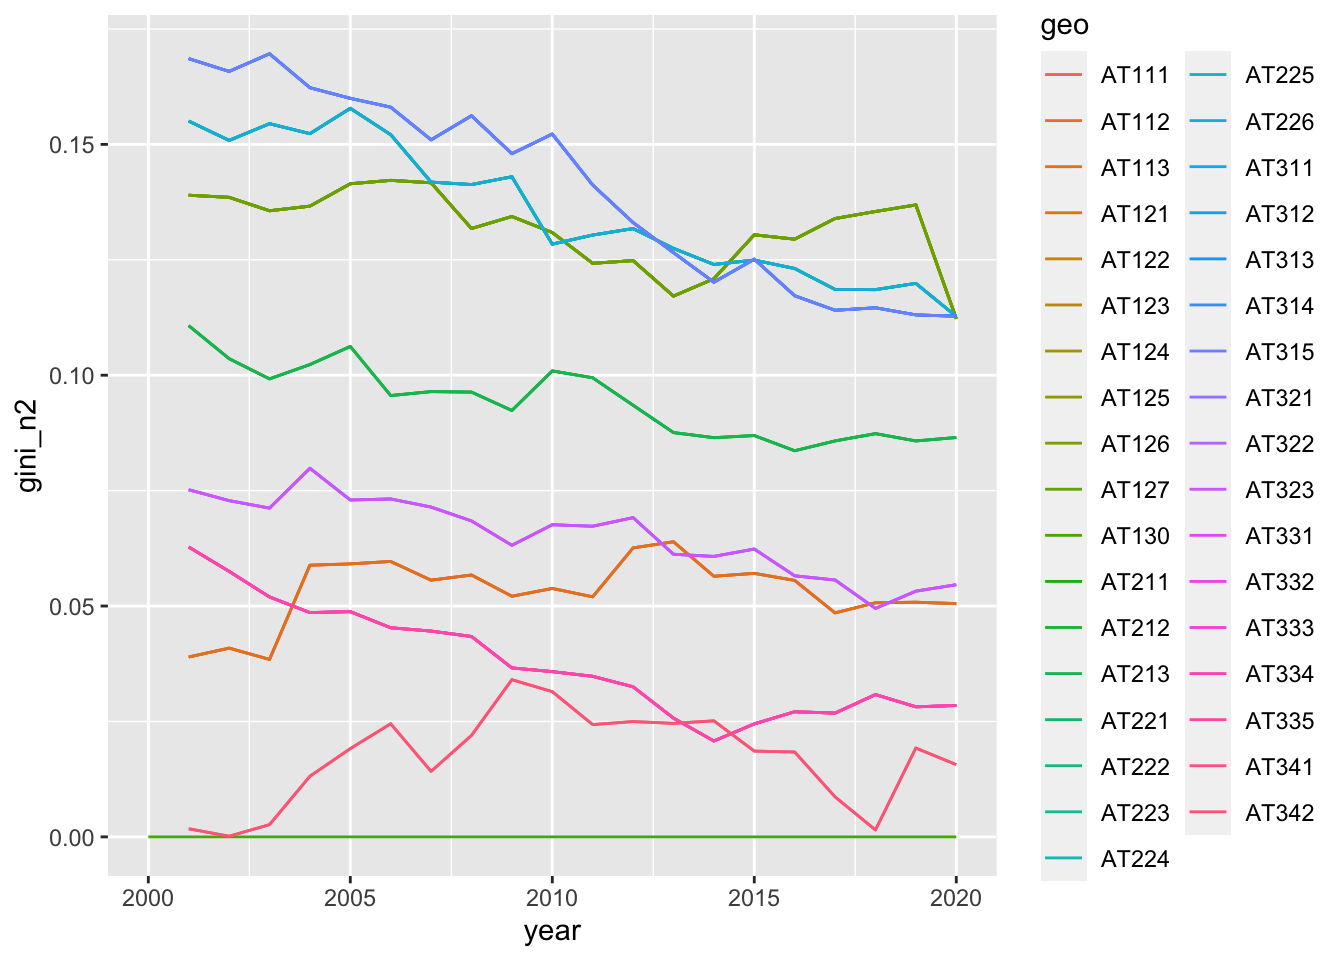
\includegraphics{assignment_1_files/figure-pdf/unnamed-chunk-29-1.pdf}

\hypertarget{outliers}{%
\subsection{Outliers}\label{outliers}}

\hypertarget{bulgaria-south-west-bg41}{%
\subsubsection{Bulgaria (South west:
BG41)}\label{bulgaria-south-west-bg41}}

The main outlier in Bulgaria the line that from 2000, was already over
15\%. This is the region BG41, also known as south west. The reason
behind this outlying difference is because the capital of Bulgaira,
Sofia, is a sub-region of BG41. In Sofia, the GDP per capita in 2020 was
nearly triple as much as the second highest sub-regions GDP per capita.

\hypertarget{italy-lombardia-itc4}{%
\subsubsection{Italy (Lombardia: ITC4)}\label{italy-lombardia-itc4}}

Lombardia has the biggest inequality in the whole of Italy, with the
highest Gini coefficient ( Gini \textgreater0.15 in 2020). ITC4 contains
big cities such as Milano, which has two of the biggest football teams
in the world, and is known for being the capital of fashion. This
attracts tourism and a spike in the regions GDP.

\hypertarget{belgium-east-flanders-be23}{%
\subsubsection{Belgium (East Flanders:
BE23)}\label{belgium-east-flanders-be23}}

Explained by the span of GDP per capita in sub-regions where the highest
GDP per capita being 49 964 and the lowest 17 401, while the average
spans between {[}17 000:21 000{]}.

\hypertarget{not-included-countries}{%
\subsubsection{Not included countries}\label{not-included-countries}}

We have not included the following countries based on a lack of
observations on level 3 data. Croatia has 140 observations , Serbia has
68 and Bosnia and Herzegovina became a EU candidate in 2022 and because
of this lacks any data.

\hypertarget{refs}{}
\begin{CSLReferences}{1}{0}
\leavevmode\vadjust pre{\hypertarget{ref-eurostat2023}{}}%
Eurostat. 2023. {``Statistics \textbar{} {Eurostat}.''}
https://ec.europa.eu/eurostat/databrowser/view/tec00115/default/table?lang=en.

\leavevmode\vadjust pre{\hypertarget{ref-lessmann2017}{}}%
Lessmann, Christian, and André Seidel. 2017. {``Regional Inequality,
Convergence, and Its Determinants \textendash{} {A} View from Outer
Space.''} \emph{European Economic Review} 92 (February): 110--32.

\end{CSLReferences}



\end{document}
